% ======================================================================
%  CleanWhite -- a sober, all-white Beamer template
%  Compile with pdflatex or lualatex (run TWICE for corner logos)
% ======================================================================
\documentclass[aspectratio=169,10pt]{beamer}

% ------------------------- PACKAGES -----------------------------------
\usepackage[T1]{fontenc}
\usepackage[utf8]{inputenc} % not needed on LuaLaTeX/XeLaTeX
\usepackage{lmodern}
\usepackage{graphicx}
\usepackage{booktabs}                 % clean tables
\usepackage{tikz}
\usepackage{svg}
\usepackage{pgfplots}
\graphicspath{{../Figures/}}
\pgfplotsset{compat=1.17}

% ======================================================================
%  EDIT ME -- presentation metadata & branding
% ======================================================================
\title[Short Title]{Full Presentation Title Goes Here}
\subtitle[Short Subtitle]{A Very Interesting and Precise Subtitle}
\author[Doe \& Smith]{Jane Doe, John Smith}
\date[09.09.2026]{September 9, 2026}

\newcommand{\ProjectName}{My Awesome Project}   % shown in footer
\newcommand{\AccentColor}{blue!65!black}        % try e.g. teal!70!black

% Corner logos (replace file names; or set \showcornerlogosfalse)
\newif\ifshowcornerlogos
\showcornerlogostrue 
\newcommand{\LogoTopRight}{\includegraphics[height=0.45cm]{MasterScienceEngineering}}
\newcommand{\LogoBottomLeft}{
\includegraphics[height=0.5cm]{HES_SO_Logo_RGB}}

% ======================================================================
%  THEME: all white, hairlines only, one accent color
% ======================================================================
\definecolor{accenthesso}{RGB}{0,96,156}
\definecolor{accentmaster}{RGB}{231,0,34}
\definecolor{textgrey}{RGB}{150,139,131}

\definecolor{accentgreen}{RGB}{0,138,94}       % vert profond, tempéré
\definecolor{accentpurple}{RGB}{110,66,166}    % violet moyenne densité
\definecolor{accentorange}{RGB}{235,126,0}     % orange chaleureux
\definecolor{accentpink}{RGB}{204,61,124}      % rose framboise
\definecolor{accentteal}{RGB}{0,140,150}        % turquoise sobre (bonus)
\definecolor{accentgold}{RGB}{176,136,0}        % doré discret (bonus)

\setbeamercolor{background canvas}{bg=white}
\setbeamercolor{normal text}{fg=black!87}
\setbeamercolor{structure}{fg=accenthesso}
\setbeamercolor{alerted text}{fg=accentmaster}
\setbeamercolor{frametitle}{fg=accenthesso}
\setbeamercolor{framesubtitle}{fg=textgrey}
\setbeamercolor{title}{fg=accenthesso}
\setbeamercolor{subtitle}{fg=textgrey}
\setbeamercolor{author}{fg=textgrey}
\setbeamercolor{date}{fg=textgrey}
\setbeamercolor{item}{fg=accenthesso!80}
\setbeamercolor{enumerate item}{fg=accenthesso!80}
\setbeamercolor{block title}{fg=accenthesso,bg=black!4}
\setbeamercolor{block body}{fg=black!80,bg=white}
\setbeamercolor{caption}{fg=textgrey}

\setbeamerfont{frametitle}{size=\large,series=\bfseries}
\setbeamerfont{framesubtitle}{size=\footnotesize}
\setbeamerfont{caption}{size=\footnotesize}
\setbeamerfont{block title}{size=\normalsize,series=\bfseries}

\setbeamertemplate{navigation symbols}{}
\setbeamersize{text margin left=0.9cm, text margin right=0.9cm}

% ---------- Frame titles (thin hairline under the title) --------------
\makeatletter
\setbeamertemplate{frametitle}{%
  \vspace*{1.5ex}%
  {\usebeamercolor[fg]{frametitle}\usebeamerfont{frametitle}\insertframetitle}%

  \ifx
    %\par\vspace{-0.1em}%
    \insertframesubtitle\@empty%
  \else%
    \par\vspace{-0.3em}%
    {\usebeamercolor[fg]{framesubtitle}\usebeamerfont{framesubtitle}\insertframesubtitle}%
    \par\vspace{-0.7em}%
  \fi%

  {\color{accenthesso!60}\rule{0.42\linewidth}{0.5pt}}%
  \par\vspace{0.1em}%
}
\makeatother

% ---------- Footline: title - subtitle - project - authors - date -----
\setbeamertemplate{footline}{%
  \leavevmode%
  \hbox{%
    \hspace*{40ex}%
    {\footnotesize\color{textgrey}%
      \insertshorttitle\;$\cdot$\;\insertshortsubtitle%
      \;$\cdot$\;\ProjectName%
      \;$\cdot$\;\insertshortauthor%
      \;$\cdot$\;\insertshortdate}%
    %\hfill%
    %{\scriptsize\color{black!75}\insertframenumber\,/\,\inserttotalframenumber}%
    %\hspace*{1.6ex}%
  }%
  \vspace*{5.7ex}%
}

% ---------- Corner logos (background canvas) ---------------------------

\makeatletter
\addtobeamertemplate{background canvas}{}{%
  % Corner logos (unchanged)
  \ifshowcornerlogos
    \begin{tikzpicture}[remember picture,overlay]
      \node[anchor=north east,inner sep=0pt]
        at ([yshift=-0.41cm,xshift=-0.68cm]current page.north east) {\LogoTopRight};
      \node[anchor=south west,inner sep=0pt]
        at ([yshift=0.4cm,xshift=0.84cm]current page.south west) {\LogoBottomLeft};
    \end{tikzpicture}%
  \fi
  % Page number pinned to the bottom-right corner
  \ifbeamer@plainframe\else
    \begin{tikzpicture}[remember picture,overlay]
      \node[anchor=south east]
        at ([xshift=-0.55cm,yshift=0.4cm]current page.south east)
        {\footnotesize\color{textgrey}\insertframenumber};
    \end{tikzpicture}%
  \fi
}
\makeatother

% ---------- Subtle bullets ---------------------------------------------
\setbeamertemplate{itemize item}{\textcolor{accenthesso!75}{\footnotesize$\bullet$}}
\setbeamertemplate{itemize subitem}{\textcolor{accenthesso!60}{\footnotesize--}}
\setbeamertemplate{itemize subsubitem}{\textcolor{textgrey}{\tiny$\bullet$}}
\setbeamertemplate{enumerate item}{\textcolor{accenthesso!80}{\footnotesize\arabic{enumi}.}}

% ---------- Custom title page ------------------------------------------
\setbeamertemplate{title page}{%
  \begin{center}
    \vspace*{1.2cm}
    {\usebeamerfont{frametitle}\usebeamercolor[fg]{title}\huge\inserttitle\par}
    \vspace{0.45em}
    {\usebeamercolor[fg]{subtitle}\large\insertsubtitle\par}
    \vspace{1.4em}
    {\color{accenthesso!60}\rule{0.3\linewidth}{0.6pt}}\par
    \vspace{1.2em}
    {\usebeamercolor[fg]{author}\insertauthor\par}
    \vspace{0.3em}
    {\small\color{textgrey}\ProjectName\par}
    \vspace{0.3em}
    {\small\color{textgrey}\insertdate\par}
  \end{center}
}

% ======================================================================
%  DOCUMENT
% ======================================================================
\begin{document}

% ------- Title page ----------------------------------------------------
\begin{frame}[plain]
  \titlepage
\end{frame}

% ------- Outline --------------------------------------------------------
\begin{frame}{Outline}
  \tableofcontents[hideallsubsections]
\end{frame}

% ------- Bullets ---------------------------------------------------------
\section{Motivation}
\begin{frame}{Why another template?}{Clean, sober, distraction-free}
  \begin{itemize}
    \item All-white background, single accent color
    \item Unobtrusive bullets and hairline separators
    \item Logos in the corners, discreet footer
      \begin{itemize}
        \item Sub-items become quiet dashes
        \item Easy to extend with your own commands
      \end{itemize}
    \item Works with figures, tables and charts
  \end{itemize}
\end{frame}

% ------- Table -----------------------------------------------------------
\section{Results}
\begin{frame}{Example table}{Measured throughput (Mbit/s)}
  \begin{table}
    \centering
    \begin{tabular}{lccc}
      \toprule
      \textcolor{accenthesso}{\textbf{Scheme}} &
      \textcolor{accenthesso}{\textbf{Load A}} &
      \textcolor{accenthesso}{\textbf{Load B}} &
      \textcolor{accenthesso}{\textbf{Gain}} \\
      \midrule
      Baseline      & 410 & 380 & --- \\
      Proposed      & 512 & 495 & +25\,\% \\
      Proposed + X  & 548 & 520 & +34\,\% \\
      \bottomrule
    \end{tabular}
  \end{table}
\end{frame}

% ------- Chart (native pgfplots) ------------------------------------------
\begin{frame}{Example chart}{Throughput over time}
  \begin{figure}
    \centering
    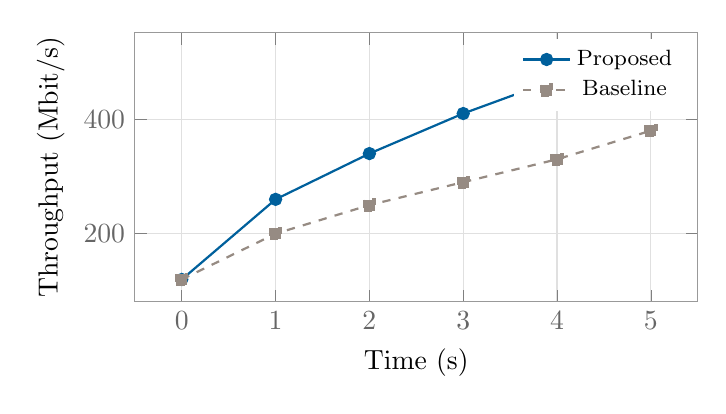
\begin{tikzpicture}
      \begin{axis}[
          width=0.72\linewidth, height=5cm,
          xlabel={Time (s)}, ylabel={Throughput (Mbit/s)},
          grid=major, grid style={black!12},
          axis line style={black!40}, tick label style={black!60},
          legend style={draw=none, font=\footnotesize},
        ]
        \addplot[accenthesso, thick, mark=*] coordinates
          {(0,120)(1,260)(2,340)(3,410)(4,470)(5,512)};
        \addplot[textgrey, thick, dashed, mark=square*] coordinates
          {(0,120)(1,200)(2,250)(3,290)(4,330)(5,380)};
        \legend{Proposed, Baseline}
      \end{axis}
    \end{tikzpicture}
    \caption{Proposed scheme versus baseline.}
  \end{figure}
\end{frame}

% ----------------------------------------------------------------------
% Color palette demo
% ----------------------------------------------------------------------
\begin{frame}{Color Palette}{Harmonized with the institutional shades}
  \begin{center}
    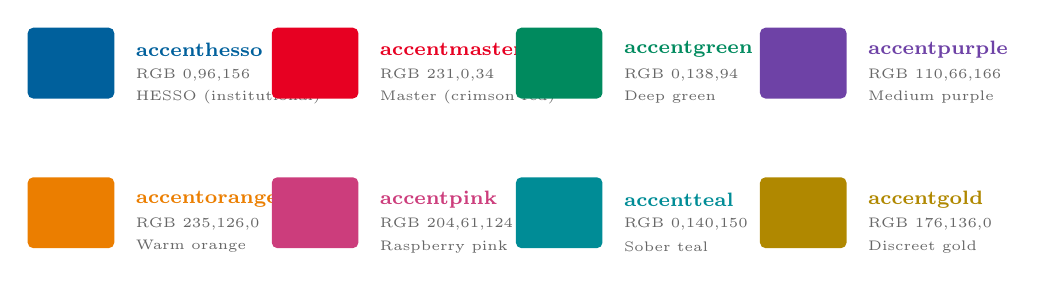
\begin{tikzpicture}
      \foreach \name/\rgb/\disp [count=\i from 0] in {
          accenthesso/{0,96,156}/{HESSO (institutional)},
          accentmaster/{231,0,34}/{Master (crimson red)},
          accentgreen/{0,138,94}/{Deep green},
          accentpurple/{110,66,166}/{Medium purple},
          accentorange/{235,126,0}/{Warm orange},
          accentpink/{204,61,124}/{Raspberry pink},
          accentteal/{0,140,150}/{Sober teal},
          accentgold/{176,136,0}/{Discreet gold}}
      {
        \pgfmathsetmacro{\row}{int(div(\i,4))}     % 0 = row 1, 1 = row 2
        \pgfmathsetmacro{\col}{int(mod(\i,4))}     % position within the row
        \begin{scope}[shift={(\col*3.1,-\row*1.9)}]
          \fill[\name, rounded corners=2pt] (0,0) rectangle (1.1,0.9);
          \node[anchor=west, text width=2.0cm, align=left]
            at (1.25,0.62)
            {\scriptsize\bfseries\textcolor{\name}{\name}};
          \node[anchor=west]
            at (1.25,0.30)
            {\tiny\color{black!60} RGB \rgb};
          \node[anchor=west]
            at (1.25,0.02)
            {\tiny\color{black!60} \disp};
        \end{scope}
      }
    \end{tikzpicture}
  \end{center}
  \vspace{0.4em}
  {\small All colors share a comparable lightness ($\approx$40--50\,\%),
   ensuring readability as text and consistency across charts --
   including grayscale printing.}
\end{frame}


% ------- External figure --------------------------------------------------
\begin{frame}{External figure}{Replace with your own graphic}
  \begin{figure}
    \centering
    \includegraphics[width=0.55\linewidth]{example-image-a}
  \end{figure}
\end{frame}

% ------- Columns ----------------------------------------------------------

\begin{frame}{Setup}{Experiment and results side by side}
  \begin{columns}[totalwidth=\textwidth]
    \begin{column}{0.5\textwidth}
      \textbf{Method}
      \begin{itemize}
        \item First condition
        \item Second condition
      \end{itemize}
    \end{column}
    \begin{column}{0.5\textwidth}
      \begin{figure}
        \includegraphics[width=\linewidth]{example-image-a}
        \caption{Result of the run.}
      \end{figure}
    \end{column}
  \end{columns}
\end{frame}

% ------- Blocks ------------------------------------------------------------
\section{Discussion}
\begin{frame}{Blocks are quiet too}
  \begin{block}{Key observation}
    Block titles are tinted light grey; bodies stay white.
  \end{block}
  \begin{alertblock}{Attention}
    Alerted blocks reuse the Master accent color.
  \end{alertblock}
\end{frame}

\end{document}